\chapter{Basic concepts in graph theory}
\label{ch:graphtheory}

Before presenting all the types of networks supported by the library, we show how basic concepts in graph theory map to library objects and functions.

\section{Graphs, vertices and edges}

\begin{definition}[Graph]
A graph G is a tuple (V, E) where V is a finite set of vertices and E is a finite set of unordered pairs of vertices (edges).
\end{definition}

In uunet, vertices and edges are objects that exist independently of a graph. The following code:

\begin{lstlisting}[style=c++]
auto v1 = make_shared<Vertex>("v");
auto v2 = make_shared<Vertex>("v");
    
auto dir = EdgeDir::UNDIRECTED;
auto edge1 = make_shared<Edge>(v1.get(), v2.get(), dir);
auto edge2 = make_shared<Edge>(v1.get(), v2.get(), dir);
\end{lstlisting}

\noindent creates the C++ objects in Figure~\ref{fig:vertices_edges-physical}. There are two Vertex objects and two Edge objects, where *v1 != *v2 even if they have the same name, and *edge1 != *edge2 even if they connect the same vertices.
These C++ objects correspond to the logical graph in Figure~\ref{fig:vertices_edges_logical}.

\begin{figure}
  \centering
\begin{subfigure}{.7\textwidth}
  \centering
  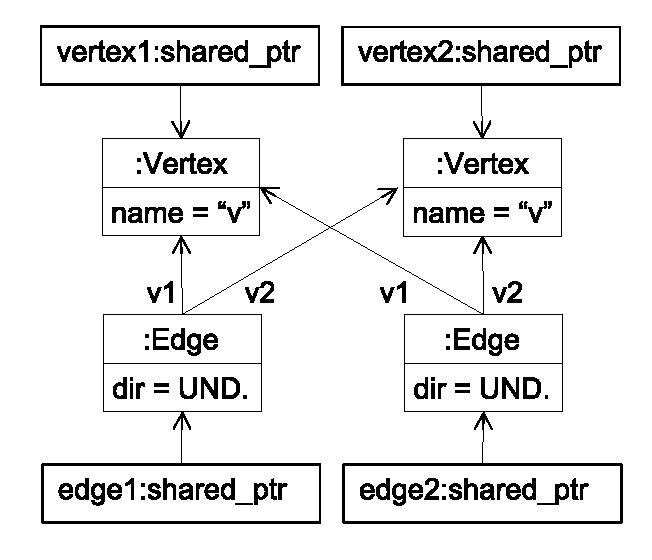
\includegraphics[width=.8\linewidth]{figs/vertices_edges_cpp.eps}
  \caption{Physical}
  \label{fig:vertices_edges-physical}
\end{subfigure}
\begin{subfigure}{.2\textwidth}
  \centering
  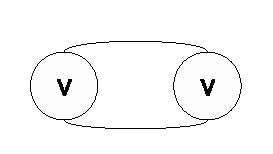
\includegraphics[width=.8\linewidth]{figs/vertices_edges_logical.eps}
  \caption{Logical}
  \label{fig:vertices_edges_logical}
\end{subfigure}
\caption{Vertices and edges: physical representation of the C++ objects and a traditional visual representation of the two vertices and edges}
\label{fig:vertices_edges}
\end{figure}

In uunet, vertices and edges may be included in a graph, where a graph:
\begin{itemize}
    \item guarantees ownership, that is, vertices and edges will keep existing at least until when they are inside some graph,
    \item allows to associate attributes to vertices and edges, that are local to the graph, and
    \item can create new vertices and edges.
\end{itemize}

\begin{figure}
    \centering
    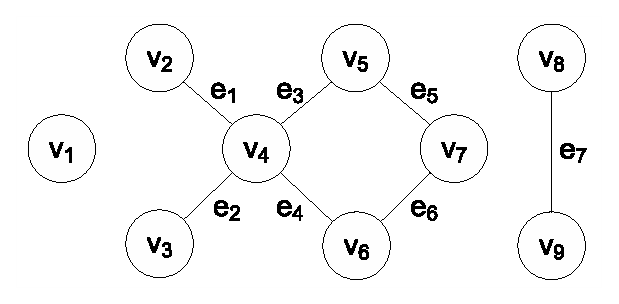
\includegraphics[width=.6\linewidth]{figs/G.eps}
    \caption{A simple graph $G$}
    \label{fig:G}
\end{figure}


To introduce basic concepts in graph theory, in this chapter we use the graph $G = (V, E)$ in Figure~\ref{fig:G}:
\begin{itemize}
    \item $ V = \{ v_1, v_2, v_3, v_4, v_5, v_6, v_7, v_8, v_9 \} $
    \item $ E = \{ e_1, e_2, e_3, e_4, e_5, e_6, e_7, e_8 \} $, where $ e_1 = (v_2, v_4)$, etc.
\end{itemize}

\begin{lstlisting}[style=c++]
// Reading the graph from file
#include "io/read_network.hpp"
const string network_file = "../simple.txt";
auto g = read_network(network_file, "G", ',');

// Vertices
auto v1 = g->vertices()->get("v1");
auto v2 = g->vertices()->get("v2");
auto v3 = g->vertices()->get("v3");
auto v4 = g->vertices()->get("v4");
auto v5 = g->vertices()->get("v5");
auto v6 = g->vertices()->get("v6");
auto v7 = g->vertices()->get("v7");
auto v8 = g->vertices()->get("v8");
auto v9 = g->vertices()->get("v9");

// Edges
auto e1 = g->edges()->get(v2, v4);
auto e2 = g->edges()->get(v3, v4);
auto e3 = g->edges()->get(v5, v4);
auto e4 = g->edges()->get(v6, v4);
auto e5 = g->edges()->get(v5, v7);
auto e6 = g->edges()->get(v6, v7);
auto e7 = g->edges()->get(v8, v9);
\end{lstlisting}

We say that:
\begin{itemize}
    \item $v_2$ and $v_4$ are \emph{end-vertices} of $e_1$.
    \item $v_2$ and $v_4$ are \emph{adjacent}.
    \item $v_2$ is a \emph{neighbor} of $v_4$, $v_4$ is a \emph{neighbor} of $v_2$.
    \item $e_1$ is \emph{incident} to $v_2$ and $v_4$.
\end{itemize}

In the following we show the corresponding code in \code{uunet}.
\begin{lstlisting}[style=c++] 
cout << "End-vertices of e1: "
    << e1->v1->name << ", " << e1->v2->name 
    << endl;
\end{lstlisting}
\begin{lstlisting}[style=out]
End-vertices of e1: v2, v4
\end{lstlisting}

\begin{lstlisting}[style=c++]
auto neigh = g->edges()->neighbors(v4);
cout << "Neighbors of v4: ";
for (auto v: *neigh)
{
    cout << v->name << " ";
}
cout << endl;
\end{lstlisting}
\begin{lstlisting}[style=out]
Neighbors of v4: v2 v3 v5 v6 
\end{lstlisting}

\begin{lstlisting}[style=c++] 
auto inc = g->edges()->incident(v4);
cout << "Edges incident to v4:" << endl;
for (auto e: *inc)
{
    cout << "(" << e1->v1->name << " -- " << e1->v2->name << ") ";
}
cout << endl;
\end{lstlisting}
\begin{lstlisting}[style=out]
Edges incident to v4:
(v2 -- v4) (v3 -- v4) (v4 -- v5) (v4 -- v6) 
\end{lstlisting}



%\section{Special types of graphs}

%Independent set: for every pair of vertices u, v ∈ V′, there is no edge in G joining the two vertices u and v.

%Bipartite graph. Partite sets.

%\section{Isomorphism}

%There is no known polynomial time algorithm to check if two graphs are isomorphic.

%\section{Walks, trails and paths}

